\chapter{Indices de vision}
	\par Nous allons maintenant présenter les différents indices placés dans la catégorie <<~vision~>>, c'est à dire les indices fournis par l'environnement immersif qui participent uniquement à la vision et non pas à l'immersion. Ces indices sont les caractéristiques perçues par un œil fixe et immobile à un instant $t$ dans le simulateur. On présente d'abord les valeurs clefs trouvables dans la littérature puis leur association à ces mêmes valeurs clefs (0, 80 et 100) du modèle, la génération de l'équation permettant d'attribuer la note entre 0 et 100 au critère et, quand c'est possible, le tracé de cette fonction.
	
	\section{Contraste \& luminosité}
	\par Le contraste est théoriquement défini comme la différence en luminosité (ou en couleur) entre les parties claires et les parties sombres d'une image ou d'un objet. Le contraste est un élément très important du système de vision humain, notamment car ce dernier est plus sensible au contraste entre deux niveaux de lumière qu'à un niveau absolu. Comme il peut être fait classiquement en psychophysique, ce stimulus peut être divisé en deux parties: sa magnitude (la valeur brute) et sa résolution (son <<~pas~>> d'évolution).
	
	\par On a pu voir les différentes approches théoriques pour le définir dans la première partie de ce manuscrit. Néanmoins il existe d'autres approches de la gestion du contraste et de la luminance comme par exemple la fonction de sensibilité ou des modèles de performance visuelle. C'est vers ces pistes qu'on s'oriente.
	
	\subsection{Fonction de sensibilité au contraste (CSF)}
	\par Les fonctions de sensibilité au contraste (CSF, pour <<~Contrast Sensibility Functions~>>) sont des courbes traçant le seuil à partir duquel l'œil humain est capable de distinguer une différence entre deux niveaux de gris. La Fig. \ref{fig:fonction_sensibilite_contraste} en est un exemple pour les trois domaines de luminosité: photopique (jour), scotopique (nuit) et mésopique (entre-deux). Tout ce qui se trouve sous la courbe est visible. Elles fonctionnent sur des mesures de seuil en cycles par degré (cpd). Les cpd sont la quantité d'alternance noir-blanc contenue dans un degré visuel.
	
	\begin{figure}
		\centering
		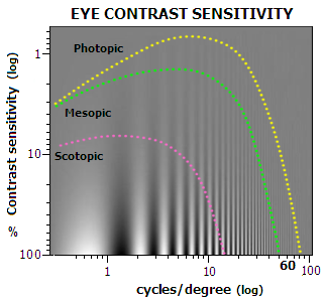
\includegraphics[scale=.9]{Figures/EyeContrastSensitivity}
		\caption{Fonctions de sensibilité au contraste pour les domaines photopiques, scotopiques et mésopiques.}
		\label{fig:fonction_sensibilite_contraste}
	\end{figure}
	
	\par Dans un premier temps, on estime que ces courbes ne sont pas suffisantes car elles ne donnent qu'un seuil en dessous duquel la perception est possible et au dessus duquel elle ne l'est pas. On ne peut en tirer aucune information sur la facilité ou la qualité de vision en dessous du seuil. Que l'on soit très proche ou très éloigné du seuil revient au même: on est dans la catégorie <<~voit~>>. On s'intéresse donc à d'autres approches sur le contraste qui nous permettraient de détailler ce qu'il se passe dans la partie visible du contraste. On s'oriente sur le concept de performance visuelle, que nous allons maintenant présenter.
	
	\subsection{Performance visuelle relative}	
	\par La performance visuelle relative (RVP - Relative Visual Performance en anglais) est définie comme la capacité du système visuel humain à réaliser une tâche donnée, capacité transposée dans une valeur numérique comprise entre 0 et 1. Les paramètres d'entrée du modèle sont en général la luminance et le contraste pour une valeur de sortie unique et sous la forme d'une valeur (comprise entre 0 et 1, donc). De nombreux modèles de performance visuelle ont été développés, notamment dans les années 80, mais deux d'entre eux peuvent être particulièrement mis en avant : le modèle de la CIE (Commission International de l'Eclairage) \citep{international_commission_on_illumination_analytic_1981} et le modèle de Rea \citep{rea_toward_1986}.
	
	\subsubsection{Modèle de la CIE}
	\par Le modèle de la CIE a été construit sur la base d'un grand nombre de résultats expérimentaux issus de nombreux chercheurs différents. Leur but était d'arriver à un outil pour aider à choisir les meilleurs conditions d'illumination pour les ateliers d'usine de manière à ce que les ouvriers travaillent au rendement maximal. En plus de la luminance et du contraste, le modèle nécessite également l'âge et le <<~niveau de demande de la tâche~>> comme paramètres d'entrée.
	
	\subsubsection{Modèles de Rea et Ouellette}
	\par Le modèle de Rea est plus simple mais ses auteurs le déclarent plus précis que celui de la CIE. Leur modèle ne prend en entrée que la luminance de la tâche et la luminance de l'arrière-plan de la tâche. Mark S. Rea présente un première version de son modèle en 1986 \citep{rea_toward_1986} puis une version raffinée en 1991 \citep{rea_relative_1991}. Dans ce dernier modèle, trois paramètres de plus ont été rajoutés: l'âge, la taille de la tâche à réaliser et la luminance d'adaptation (quantité de lumière à laquelle les yeux ont adapté la taille de leur pupille). Ce modèle permet de tracer les graphes visibles en Fig. \ref{fig:courbes_rea}. Ces courbes représentent la performance visuelle en fonction de la luminosité et du contraste pour une taille d'objet vu donnée: la courbe de gauche, plus prononcée, concerne un objet plus petit que celui pour la courbe de droite, moins prononcée.
	
	\begin{figure}
		\centering
		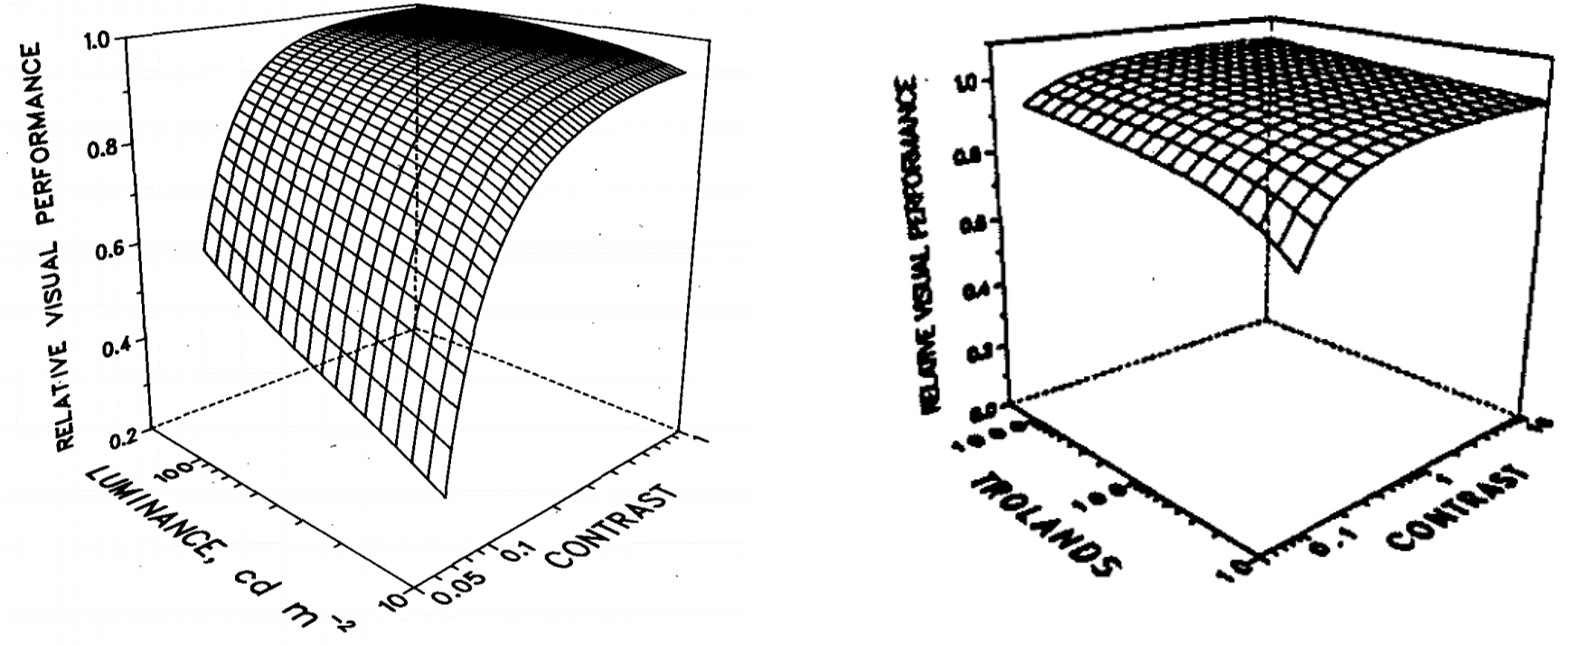
\includegraphics[scale=.5]{Figures/CourbesReaExemple}
		\caption{Exemple de performance visuelle pour deux tailles de cible différentes}
		\label{fig:courbes_rea}
	\end{figure}
	
	\subsubsection{Vers une vérification expérimentale}
	\par Néanmoins, ces deux modèles n'ont pas été pensés pour la Réalité Virtuelle et pourraient ne pas s'inscrire dans pour une utilisation directe dans notre modèle de score de réalisme, en lieu et place du critère de luminance et de contraste. Une expérimentation a été réalisée pour confirmer ou infirmer cette hypothèse, notamment à propos du modèle de Rea (voir partie suivante). L'objectif serait de mettre à l'échelle entre 0 et 100 les résultats entre 0 et 1 du modèle de performance visuelle. Il est à noter que dans son modèle la CIE définit la valeur de 0.8 (80 ramené à notre échelle) comme la performance standard.
	
	\section{Images par seconde}	
	\par Attribuer des valeurs spécifiques, discrètes, aux phénomènes qui composent la vision peut sembler peu naturel tant le processus de vision est continu \citep{bear_neurosciences:_2007}. Néanmoins, c'est un exercice auquel on se risque et il existe un certain nombre d'effets notables qui n'apparaissent qu'à certains nombres d'images par seconde (frame rate).
	
	\subsection{Minimum de fonctionnement}
	\par Premièrement, la perception du mouvement n'est pas basée (comme cela a été suspecté pendant longtemps) sur la persistance rétinienne mais sur deux illusions perceptuelles: l'effet \textit{phi} et le mouvement \textit{bêta} \citep{de_lauretis_flicker_1980}. La persitance rétinienne est un phénomène passif laissant une image rémanente sur la rétine pendant un court instant. L'effet phi est une illusion de mouvement, cette fois active, dans le cerveau et le traitement des images, pour un système en boucle fermée. Le mouvement bêta est lui aussi une illusion d'optique active mais pour les système ouverts. Ces effets sont illustrés en Fig. \ref{fig:beta_phi}). Ils apparaissent à partir de 16 images par seconde. En dessous de cette valeur, aucun mouvement n'est perçu, seulement une suite distincte d'images.
	
	\begin{figure}
		\centering
		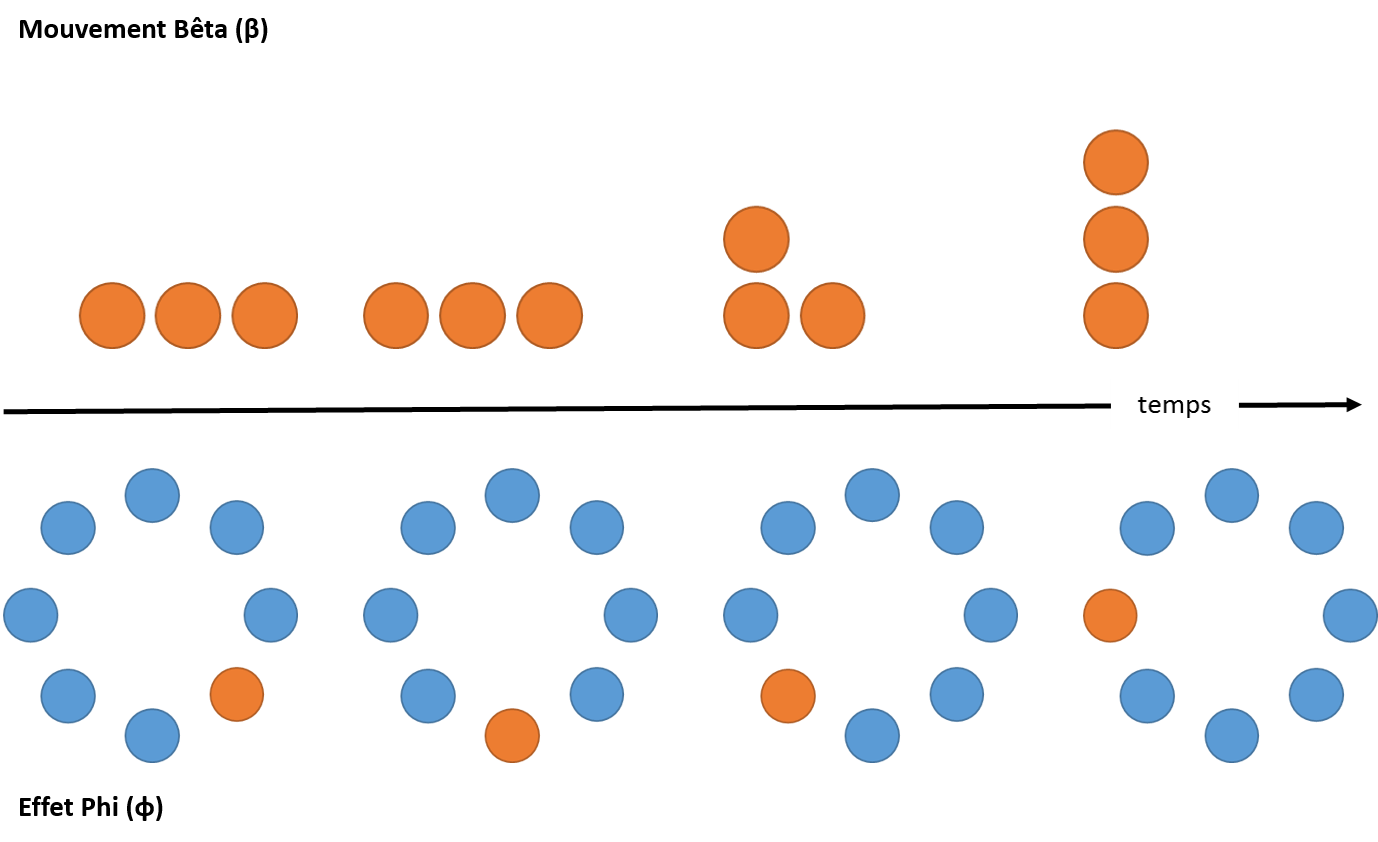
\includegraphics[scale=.55]{Figures/MouvementBetaEffetPhi}
		\caption{Illustration du <<~mouvement beta~>> et de l'<<~effet phi~>>}
		\label{fig:beta_phi}
	\end{figure}
	
	\subsection{Phénomène de scintillement (flickering)}
	\par Deuxièmement, un autre grand phénomène induit par la vision en informatique est le <<~flickering~>>, le clignotement/scintillement de l'écran. Ce phénomène intervient quand le frame rate est trop lent et que l'œil devient capable de percevoir un effet de diminution/changement de luminosité (fading) entre les images. Driscoll \citep{driscoll_eyes_1978}, en s'appuyant sur les travaux de Landis \citep{landis_determinants_1954} et de de Lange \citep{de_lange_dzn_research_1958,de_lange_dzn_research_1958-1}, a travaillé sur la détermination de la fréquence critique de clignotement pour l'œil, c'est à dire la fréquence au delà de laquelle le cerveau ne perçoit plus de clignotement. La fréquence critique de clignotement semble être basée sur un ratio appelé <<~ratio d'ondulation~>> ou <<~ratio ondulatoire~>> (\textit{ripple ratio} en anglais) qui se calcule de la manière suivante (Eq. \ref{eq:ripple_ratio}):
	
	\begin{equation}
	r = \frac{\textrm{Amplitude de l'harmonique fondamentale}}{\textrm{Luminance moyenne}}
	\label{eq:ripple_ratio}
	\end{equation}
	
	\par En utilisant les courbes établies par Driscoll, les courbes de la fonction de transfert de modulation temporelle, quel que soit le ratio ondulatoire, c'est à dire quelle que soit la nature de l'onde lumineuse, la fréquence critique de clignotement, quelle que soit la luminance, est de 70~Hz.
	
	\subsection{Maximum de fonctionnement}	
	\subsubsection{L'hypothèse des deux voies}
	\par D'autres valeurs viennent des voies dorsale et ventrale. Pour rappel, la théorie des deux voies est le postulat principal permettant d'expliquer la manière dont le cerveau traite les informations visuelles arrivant des nerfs optiques. Une fois dans le cerveau, l'information est divisée en deux boucles de traitement \citep{ingle_two_1982,dhondt_emotion_2011}. La première, la voie dorsale ou pariétale, est la boucle <<~où~>> et s'occupe d'extraire la direction et le mouvement du flux d'image qui arrive. L'autre voie, la voie ventrale ou temporale, dite boucle du <<~quoi~>>, s'occupe d'extraire la forme, la couleur et la texture. Les deux voies fonctionnent supposément à des fréquences autour de, respectivement, 200~Hz et 25~Hz, ce qui est corrélé par le fait que l'une est rapide et l'autre lente \citep{dhondt_emotion_2011}, par le nombre de cortex différents par lesquels ces voies passent \citep{dhondt_emotion_2011} et par les latences propres de chaque cortex \citep{bullier_integrated_2001} ; cependant, aucunes valeurs précises n'ont été scientifiquement établies.
	
	\subsubsection{Les pilotes de l'US Air Force}	
	Parallèlement, l'US Air Force aurait conduit des expériences sur ses pilotes de chasse pendant lesquelles ceux-ci étaient capables de reconnaitre un modèle d'avion sur des images flashées à 1/220ème de seconde\footnote{Human Eye Frames Per Second. Dans \textit{AMO.net America's Multimedia Online}. Vu sur \url{http://amo.net/nt/02-21-01fps.html}}. Même si cela ne constitue pas une preuve scientifique en tant que telle, cela vient renforcer l'hypothèse des deux voies sur la fréquence maximale associable au traitement visuel. A la différence du minimum de fonctionnement où des phénomènes sont clairement établis avec des fréquences de fonctionnement claires, on ne peut ici fonctionner que sur des approximations.
		
	\subsection{Fonction de notation du critère}
	\par Ainsi, en utilisant les trois valeurs clefs précédemment présentées: le nombre minimal de fréquence d'image pour percevoir le mouvement (16~Hz), la fréquence critique de clignotement (70~Hz) et la fréquence supposée de la voie dorsale (200~Hz), on peut assembler un modèle mathématique et en tirer une courbe. Dans le cas de ce critère, avec $f$ le nombre d'images par seconde du système de visualisation, on présente l'équation suivante (Eq. \ref{eq:fps_score}), dont le tracé est donné en Fig. \ref{fig:score_fps}:
	\begin{equation}
		F_{FPS}(f) = \begin{cases}
		0 & f < 16\\
		126.5 - \frac{367.1}{\sqrt{f - 7.6}} & sinon\\
		100 & f > 200
		\end{cases}
		\label{eq:fps_score}
	\end{equation}

	\begin{figure}
		\centering
		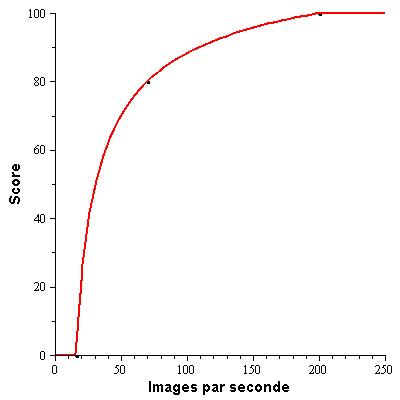
\includegraphics[scale=.75]{Figures/FPS}
		\caption{Tracé de la fonction de notation du critère <<~images par seconde~>>}
		\label{fig:score_fps}
	\end{figure}

	\par Finalement, il doit être noté que toutes ces valeurs clefs sont définies pour un œil unique et donc qu'elles doivent être multipliées par deux dans le cas d'une application à la VR utilisant la stéréoscopie active (c'est à dire avec une image sur deux présentée à chaque œil) pour une imagerie 3D. %De plus, ces fréquences sont les nombres d'images par seconde effectifs, c'est à dire ceux qui sont réellement affichés par l'écran et non pas les nombres d'images par seconde du hardware (en sortie de carte graphique par exemple) qui sont en général plus élevés à cause du principe de Shannon (plusieurs occurrences d'un signal sont nécessaires pour son échantillonnage).
	
	\section{Couleurs}
	\subsection{Dénombrement des couleurs visibles}	
	\par La première approche serait d' essayer d'estimer le nombre de couleurs réellement visibles (discernables) par un œil humain. Cette entreprise a été tentée un certain nombre de fois \citep{kuehni_how_2015, linhares_number_2008, perales_calculation_2008, pointer_gamut_1980, pointer_number_1998, wen_display_2006} sans jamais faire preuve de beaucoup de succès: les estimations varient entre 100.000 et 10 millions de couleurs visibles.
	
	\par Les estimations se font mathématiquement: soit en utilisant les équations de différentiation des couleurs, soit en recalculant des observateurs réels pour les comparer à l'observateur idéal établi par la CIE (voir la première partie et le chapitre sur la couleur).
	
	\subsection{Les espaces colorimétriques}
	\par A défaut d'avoir une estimation validée du nombre de couleurs perceptibles et de pouvoir proposer une méthode pour calculer facilement ce même nombre dans un simulateur pour ensuite les comparer, on se tourne vers les espaces colorimétriques.
	
	\par En 1931, la Commission Internationale de l'Eclairage (CIE) a établi la définition de l'espace colorimétrique RGB. Cet espace de couleur représente l'ensemble des couleurs (non dénombrées) qui peuvent être vues par un observateur normal possédant les trois types de cônes. Cependant, il n'existe encore aucune technique pour afficher 100\% des couleurs théoriquement incluses dans l'espace RGB. Chaque système utilise une fraction de cet espace de couleur qu'on appelle <<~gamut~>> et qui dépend de trois (ou plus suivant les espaces) couleurs primaires choisies spécifiquement par la norme (Fig. \ref{fig:multi_gamut}). Dans la table suivante (Table. \ref{tab:gamut}), on présente un certain nombre de normes avec la proportion d'espace colorimétrique couverte par leur gamut. Il est à noter que dans le cas de la norme ProPhoto RGB, 13\% des couleurs atteignables sont en fait des couleurs imaginaires à cause de couleurs primaires qui sont prises hors de l'espace RGB de 1931. Empiriquement, l'acceptation commence à partir d'Adobe RGB.

	\begin{table}[h]	
		\centering
		\caption{Gamuts Coverage of 1931 Color Space}
		\label{tab:gamut}
		\small
		\begin{tabular}{ll}
			BR.709 (HDTV) & 35.9\%\\
			Adobe RGB & 52.1\%\\
			Digital Cinema & 53.6\%\\
			BT.2020 (UHD) & 75.8\%\\
			Wide-Gamut RGB & 77.6\%\\
			ProPhoto RGB & 90.0\%\\
		\end{tabular}
	\end{table}
	
	\begin{figure}
		\centering
		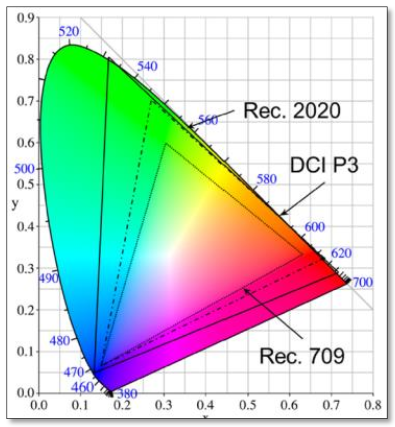
\includegraphics[scale=.9]{Figures/GamutBT2020}
		\caption{Tracé de différents gamuts sur l'espace colorimétrique CIE RGB 1931.}
		\label{fig:multi_gamut}
	\end{figure}
	
	\subsection{Indice de rendu des couleurs (IRC)}
	\par La piste de l'indice de rendu des couleurs (IRC) est une piste élégante, qui, à l'instar du critère de contraste et de luminosité propose une méthode donnant directement une valeur entre 0 et 1 et donc transposable au score de réalisme.
	
	\par Néanmoins, l'IRC est une valeur qui compare le spectre lumineux d'une lampe (dans notre cas, cela pourrait être un projecteur dans un simulateur) avec le spectre d'une lampe de référence, sensé être complet. Il y a donc principalement deux problèmes qui nous empêchent d'implémenter cette solution dans notre modèle: l'indice est dévolu aux lampes et non aux écrans, ce qui restreindrait le champ d'action de notre score de réalisme ; et surtout, la comparaison est faite par rapport à une lampe idéale et non par rapport au système visuel humain. On laisse donc de côté cette piste pour revenir à une modélisation plus simple mais plus proche de l'objectif fixé de proximité avec le système visuel humain. 
	
	\subsection{Fonction de notation du critère}
	\par Notre proposition de notation pour le critère de couleur est donc réduite à une fonction linéaire entre le score et le pourcentage de couverture de l'espace RGB 1931 auquel le système peut prétendre (Fig. \ref{fig:score_color}). Ce pourcentage vient directement de-s espace-s colorimétrique-s impliqué-s dans la chaine de rendu et d'affichage. La fonction de score pour ce critère est donc, avec $c$ le pourcentage de couverture de RBB 1931 par le gamut:
	 \begin{equation}
		F_{color}(c) = \begin{cases}
		c &\\
		100 & c > 100
		\end{cases}
		\label{eq:color}
	\end{equation}
	
	\par Il pourrait être intéressant de réaliser une expérimentation sur les besoins en couleurs (à différentier de l'appréciation du nombre de couleurs) en comparant par exemple des populations novices avec des populations expertes. Néanmoins faute de temps et de moyens (aujourd'hui encore aucun appareil commercial n'est capable d'afficher l'intégralité de l'espace RGB 1931) ce ne sera pas réalisable le temps de la thèse.
	
	\begin{figure}
		\centering
		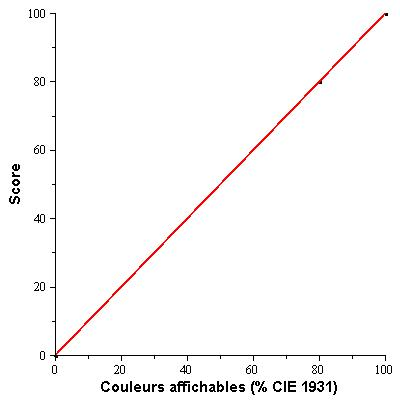
\includegraphics[scale=1]{Figures/Color}
		\caption{Tracé de la fonction de notation du critère <<~couleurs~>>}
		\label{fig:score_color}
	\end{figure}
	
	\section{Champ de vision}
	\par Le champ de vision (FOV - Field of View en anglais) est défini comme la portion d'espace qu'une personne peut voir à un instant t, sans bouger la tête. Il ne doit pas être confondu avec le champ de regard (FOR - Field of Regard en anglais) qui est la portion d'espace totale que l'on peut voir au cours du temps lorsque les mouvements de la tête et des yeux sont pris en compte.

	\par Le champ de vision se décompose en deux orientations: l'axe vertical et l'axe horizontal. On propose deux ensembles de valeurs, un par axe, pour la notation. Les deux axes seront ensuite pondérés l'un par rapport à l'autre. On fait l'hypothèse dans un premier temps que cette pondération se fait par rapport à leur taille respective. La valeur du champ de vision que l'on mesure pour introduire dans le score doit être prise pour la position standard du sujet dans l'environnement immersif (que ce soit la position du corps ou l'orientation de la tête).
	
	\subsection{Axe horizontal}
	\par Certaines des valeurs les plus communes admises pour le champ de vision horizontal sont recensées chez \citep{devisme_optimisation_2004}. Sur l'angle d'azimut (horizontal), avec les deux yeux, un être humain normal peux voir sur 170 à 190 degrés. A l'intérieur de cet angle d'azimut, seuls 120 degrés (centrés) permettent de voir binoculairement. La vision binoculaire est possible grâce à la superposition des portions d'espace vues par chaque oeil simultanément. L'acuité maximale est atteinte dans la zone fovéale soit entre 3 et 5 degrés de portion d'espace, au centre de la vision. La lecture n'est possible que dans un angle de 20 degrés tandis que la reconnaissance des formes est possible jusqu'à 40 degrés et la reconnaissance des couleurs jusqu'à 60 degrés. Ces différentes valeurs sont résumées dans la Fig. \ref{fig:champ_vision_horizontal}. L'équation propre à l'axe horizontal est, avec $h$ la valeur en degrés du champ de vision horizontal (H-FOV) calculé dans le système immersif (Eq. \ref{eq:score_h_fov}):
	\begin{equation}
	F_h(h) = \begin{cases}
		0 & h < 20\\
		19.6 \sqrt{h} -0.5 \cdot h -78.3 & sinon\\
		100 & h > 180
	\end{cases}
	\label{eq:score_h_fov}
	\end{equation}
	
	\begin{figure}
		\centering
		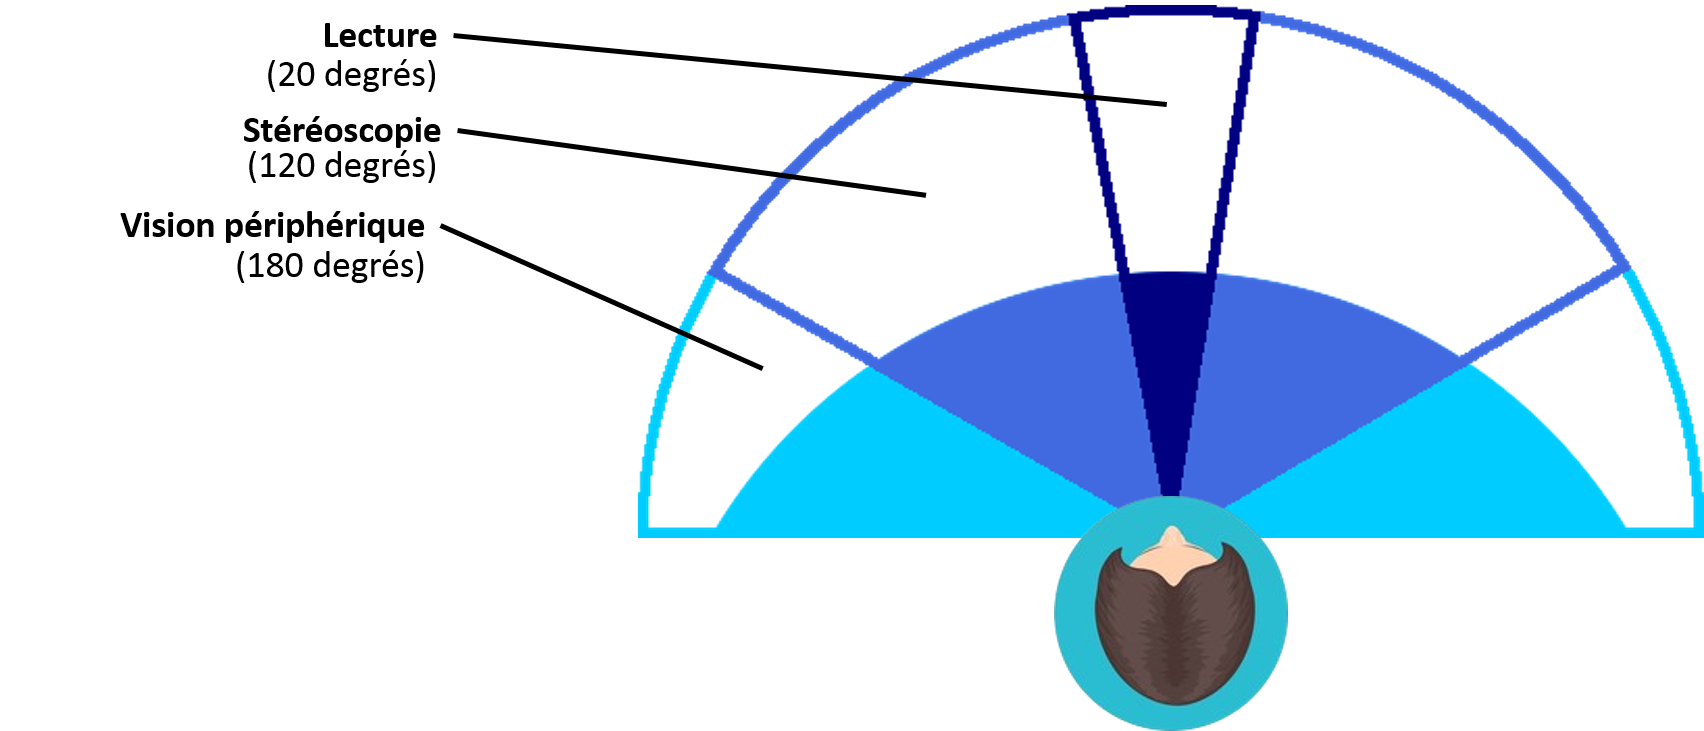
\includegraphics[scale=.5]{Figures/ChampVisionHorizontal}
		\caption{Répartition des zones visuelles sur l'axe horizontal du champ de vision.}
		\label{fig:champ_vision_horizontal}
	\end{figure}

	\subsection{Axe vertical}
	\par On retient trois valeurs caractéristiques parmi les nombreuses qu'on peut trouver dans la littérature pour le champ de vision vertical. La première correspond à la totalité de la vision latérale sur l'axe vertical: 130 degrés. On retient aussi les angles d'impression induite (85 degrés) et de vigilance (20 degrés) \citep{langlois_adas_2013} (Fig. \ref{fig:champ_vision_vertical}). L'équation propre à l'axe vertical est, avec $v$ la valeur en degrés du champ de vision vertical (V-FOV) (Eq. \ref{eq:score_v_fov}): 
	\begin{equation}
	F_v(v) = \begin{cases}
	0 & v < 20\\
	32.0 \sqrt{v} -1.1 \cdot v -121.1 & sinon\\
	100 & v > 130
	\end{cases}
	\label{eq:score_v_fov}
	\end{equation}
	
	\begin{figure}
		\centering
		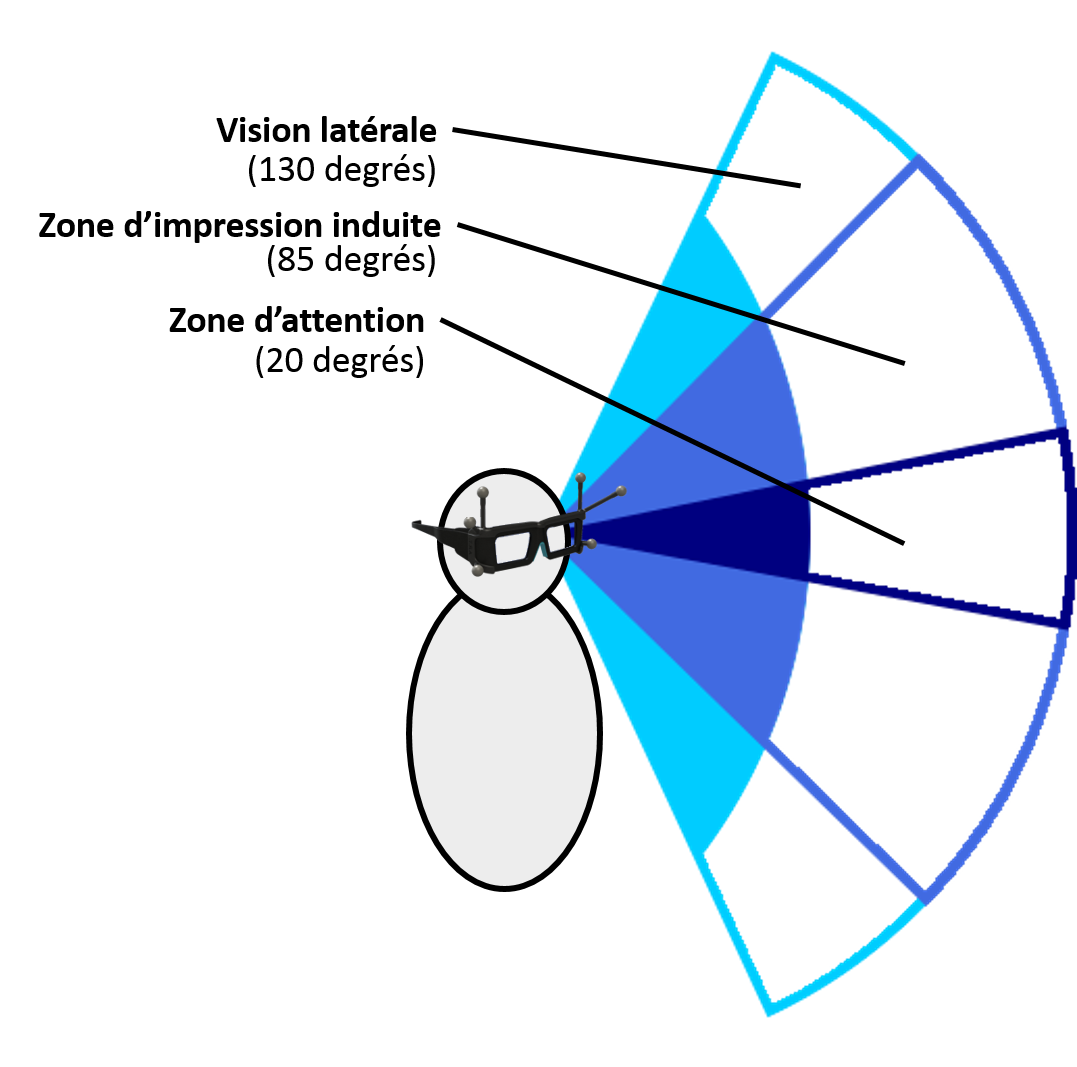
\includegraphics[scale=.6]{Figures/ChampVisionVertical}
		\caption{Répartition des zones visuelles sur l'axe vertical du champ de vision.}
		\label{fig:champ_vision_vertical}
	\end{figure}
	
	\subsection{Pondération}
	\par On pose notre propre hypothèse d'égale importance des axes verticaux et horizontaux dans le champ de vision. Cette hypothèse est une sorte de <<~cas général~>>. On verra par la suite que l'on sera amené à la modifier. On pondère donc les deux sous-critères en fonction de leur taille maximale respective (180 degrés pour l'axe horizontal et 130 pour l'axe vertical) (Eq. \ref{eq:coeff_fov}):
	\begin{equation}
		\begin{cases}	
			k_h = \frac{180}{180 + 130} = 0.58\\
			k_v = 1 - k_h = 0.42
		\end{cases}
		\label{eq:coeff_fov}
	\end{equation}
	
	\subsection{Fonction de notation du critère}
	\par Au final, la fonction de notation du critère de champ de vision est l'agrégation des précédentes équations via une pondération et s'apparente comme suit (Eq. \ref{eq:score_fov}):
	\begin{equation}
	F_{FOV}(h,v) = k_h \cdot F_h(h) + k_v \cdot F_v(v)
	\label{eq:score_fov}
	\end{equation}

	\begin{figure}
		\centering
		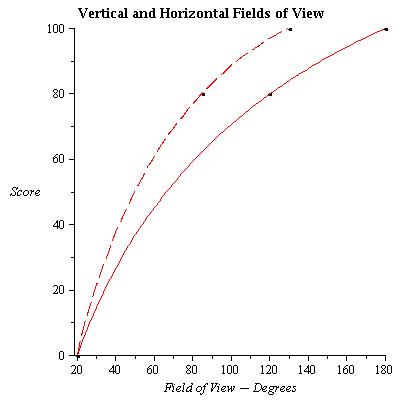
\includegraphics[scale=1]{Figures/FOV}
		\caption{Tracé de la sous-fonction horizontale de notation du critère <<~champ de vision~>> (ligne continue) et de la sous-fonction verticale (pointillés).}
		\label{fig:score_fov}
	\end{figure}
	
	\section{Acuité monoscopique}
	
	\subsection{Première approche}	
	\par Notre première approche était de se raccrocher à un tableau établi par la <<~classification internationale des maladies~>> (CIM), publié par l'Organisation Mondiale de la Santé (OMS). L'objectif est de permettre l'analyse systématique des maladies et autres affections du corps. On s'intéresse ici à la partie relative aux trouble de la vision et plus particulièrement à l'acuité. On utilise la version cliniquement modifiée de la 9ème révision de cette classification, ICD-9-CM, sortie en 1975. La 10ème révision, ICD-10 ne faisant pas encore l'unanimité et ne rajoutant que d'autres entrées sans modifier celle ci.
	
	\par La Fig. \ref{fig:icd_9_cdm} montre les différentes acuités possibles pour l'œil humain (encadré en bleu), associées avec le type de vision et surtout un score équivalent (encadré en bleu). Ce score est néanmoins peu adapté à notre utilisation, d'abord parce qu'il dépasse la note de 100 mais surtout parce qu'il englobe des acuités bien trop faibles pour être transposées en taille de pixel dans un simulateur. De plus il correspond à des défauts de vision plus qu'à des capacités de vision. On s'oriente alors vers une autre approche.
	
	\begin{figure}
		\centering
		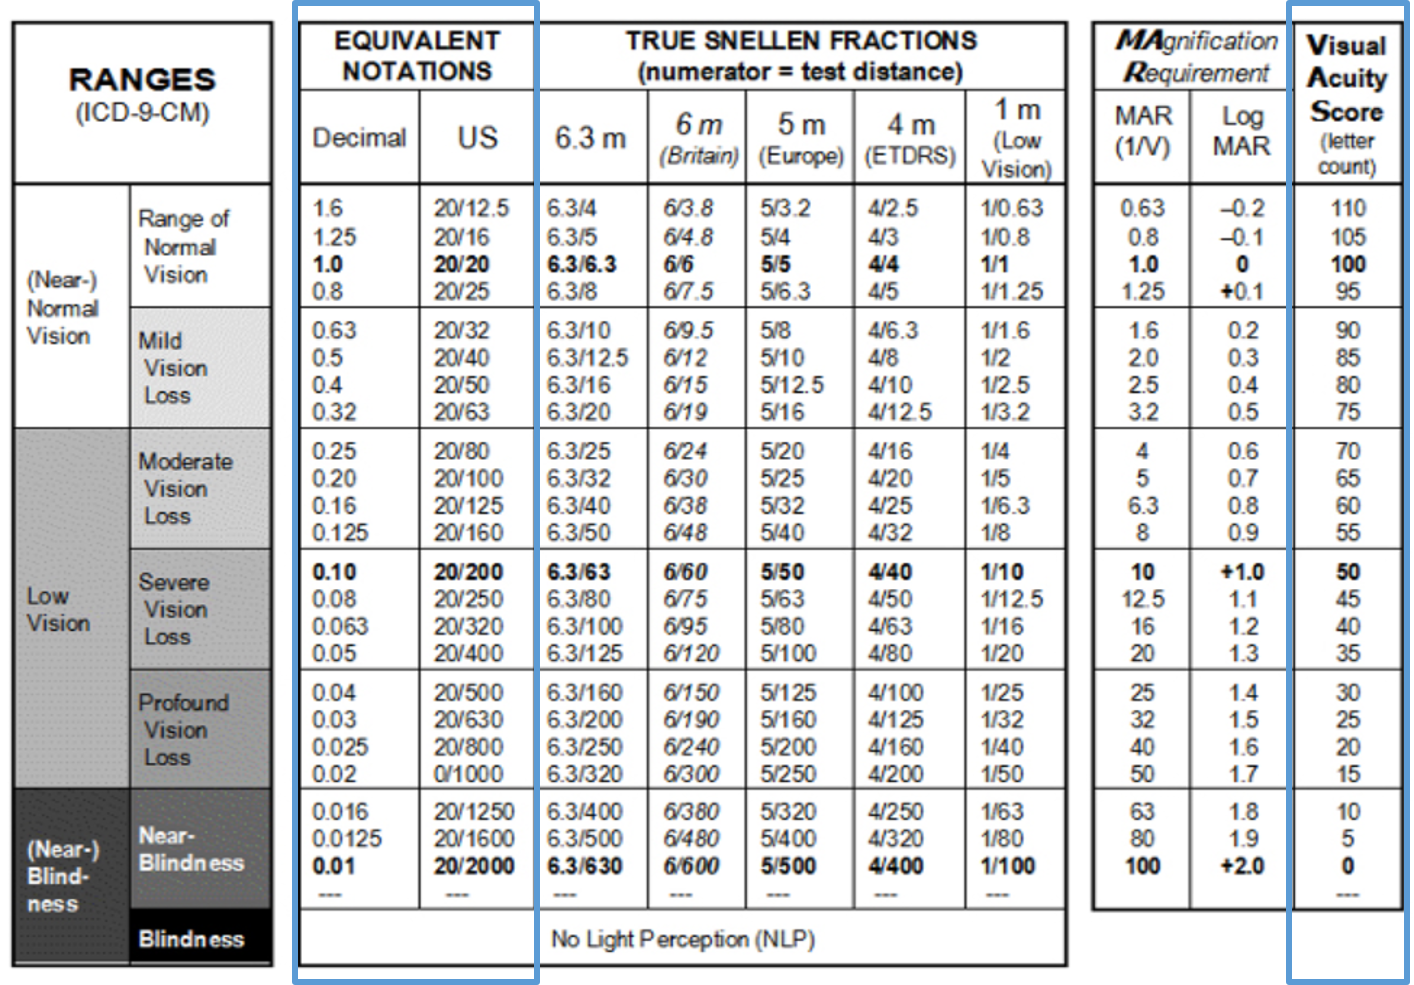
\includegraphics[scale=.6]{Figures/AcuityICD9CM}
		\caption{Classification ICD-9-CM}{On cherche à établir un lien entre les colonnes encadrées: l'acuité, et le score.}
		\label{fig:icd_9_cdm}
	\end{figure}
	
	\subsection{Deuxième approche}
	\par L'acuité monoscopique est la précision de l'œil humain, sa résolution ; c'est à dire à quel point la plus petite chose qui peut être vue peut être petite ou bien quelle est le plus petit écart perceptible entre deux motifs. Ce concept peut être directement lié à la taille du pixel sur un écran: plus le pixel est petit plus l'image est précise. Néanmoins, à partir d'une certaine taille, le pixel devient plus petit que la résolution de l'œil et devient alors non-discernable individuellement, et donc, pas forcément très utile.
	
	\par Habituellement, on estime que le système visuel humain a une acuité monoscopique comprise entre 30 secondes d'arc et 2 minutes d'arc, avec une moyenne à 1 minute d'arc \citep{fuchs_traite_2003}. Ces valeurs peuvent être, dans des conditions photopiques d'éclairage, raffinées en fonction de la tâche \citep{gross_human_2008} (voir Tab. \ref{tab:acuity}).

	\begin{table}[h]
		\centering
		\caption{Acuité de l'œil, \citep{gross_human_2008}}
		\label{tab:acuity}
		\small
		\begin{tabular}{ll}
			\multicolumn{1}{c}{\bfseries Task} & \multicolumn{1}{c}{\bfseries Acuity}\\
			Reconnaissance de forme & 5'\\
			Résolution d'une grille & 2'\\
			Résolution deux points (couleurs identiques) & 1'\\
			Résolution deux points (couleurs inversées) & 30"\\
			Acuité de Vernier (fines lignes droites parallèles) & 10"\\
			Acuité stéréoscopique & 5"\\
		\end{tabular}
	\end{table}
	
	\par La résolution de Vernier n'est atteignable que dans certaines conditions spécifiques et l'acuité stéréoscopique est un sujet à part, traité avec une autre approche, décrite dans la section suivante. De plus, Deering a montré que la plus petite résolution possible sur un écran est de 28 secondes d'arc \citep{deering_limits_1998}. C'est pourquoi on ne retient que les valeurs entre 5 minutes d'arc et 30 secondes d'arc.
	
	\subsection{Fonction de notation du critère}
	\par L'équation qui est proposée depuis ces valeurs, avec $\alpha$ l'angle sous lequel le pixel est vu, en minute d'arc (Eq. \ref{eq:mono_acuity_score}, tracé en Fig. \ref{fig:score_mono_acuity}) est la suivante:
	
	\begin{equation}
		F_{acuite\_mono}(\alpha) = \begin{cases}
		0 & \alpha > 3.5\\
		128.9 - 68.8 \sqrt{\alpha} - \frac{0.1}{\alpha} & sinon\\
		100 & \alpha < \frac{1}{6}
		\end{cases}
		\label{eq:mono_acuity_score}
	\end{equation}

	\begin{figure}
		\centering
		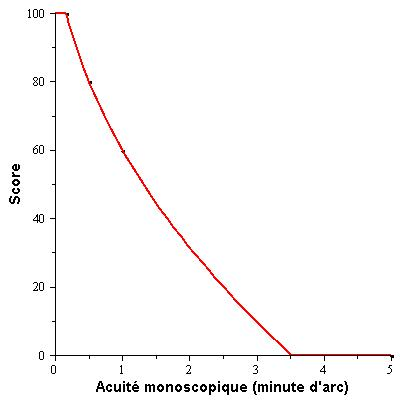
\includegraphics[scale=.75]{Figures/AcuityMono}
		\caption{Tracé de la fonction de notation du critère <<~acuité monoscopique~>>}
		\label{fig:score_mono_acuity}
	\end{figure}
	
	\section{Acuité stéréoscopique}
	\subsection{Première modélisation}	
	\subsubsection{Modèle usuel}	
	\par L'acuité stéréoscopique est la capacité du système visuel humain à percevoir une différence de profondeur entre deux plans, à une distance donnée. C'est une caractéristique qui est largement connue et décrite dans la littérature. Sa description mathématique vient d'une analyse géométrique simple \citep{fuchs_traite_2003,gross_human_2008}. Le modèle globalement accepté est le suivant (Eq. \ref{eq:stereo_model}):

	\begin{equation}	
		\Delta r = 0.001 \times r^2
		\label{eq:stereo_model}
	\end{equation}
	 
	\par Avec $\Delta r$ la différence minimale théorique de différence en profondeur (en millimètres) et $r$ la distance d'observation en mètres. Le facteur 0.001 est le rapport entre le seuil physiologique de la vision stéréoscopique ($\Delta \nu_{min}$) et la distance inter-pupillaire (DIO).
	
	\subsubsection{Limites et solution d'amélioration}
	\par Cependant, ces deux derniers paramètres peuvent varier de manière significative: la distance inter-pupillaire varie de 52 à 78~mm sur toute la population \citep{dodgson_variation_2004} (Fig. \ref{fig:variation_dio_population}) tandis que le seuil physiologique de vision dépend de la luminance, notamment quand celle ci est à un niveau très bas \citep{gross_human_2008}. On peut néanmoins conserver la valeur de 0.001 comme constante dans le modèle car la variation suivant les deux paramètres est assez faible (Fig. \ref{fig:variation_constante_dio}).
	
	\begin{figure}
		\centering
		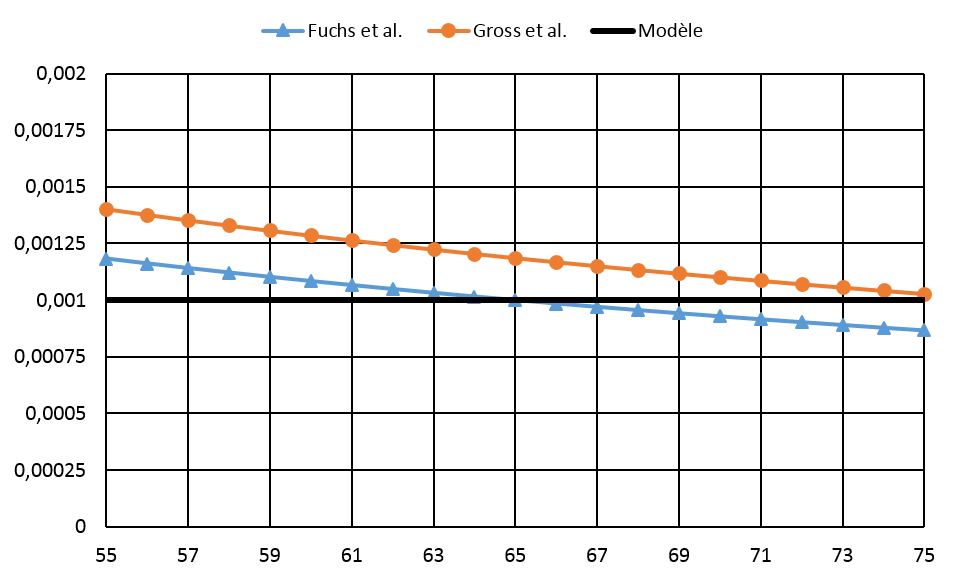
\includegraphics[scale=1]{Figures/FractionVariation}
		\caption{Variation de la constante du modèle d'acuité stéréoscopique en fonction de la distance interoculaire.}
		\label{fig:variation_constante_dio}
	\end{figure}
	
	\begin{figure}
		\centering
		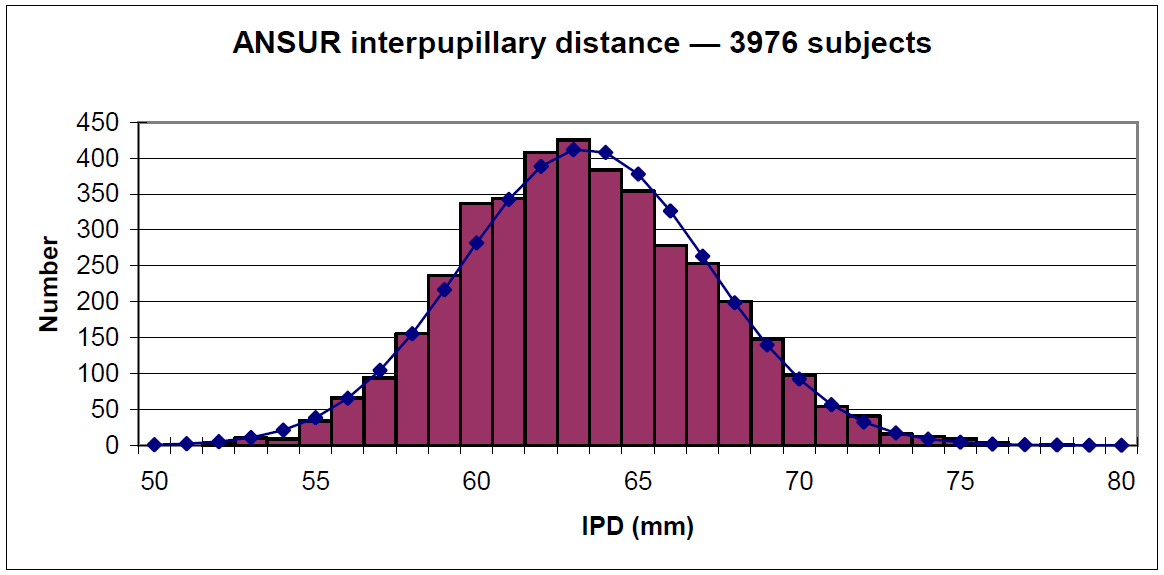
\includegraphics[scale=.5]{Figures/ANSURIPD}
		\caption{Variation de la distance interoculaire sur la population. Image tirée de \citep{dodgson_variation_2004}}
		\label{fig:variation_dio_population}
	\end{figure}
	
	\par De plus, un processus standardisé pour mesurer la valeur de $\Delta r$ d'un système serait difficile à mettre en place car il faudrait faire passer un test à un certain nombre de sujets puis en extraire le seuil moyen expérimental, ce qui sort du cahier des charges du score de réalisme. En travaillant la relation qui décrit ce même modèle d'acuité stéréoscopique (Eq. \ref{eq:limiting_angle}) \citep{gross_human_2008}, le seuil physiologique de vision apparait comme une valeur essentielle pour la vision stéréoscopique tout en étant reliée à la fois au système visuel humain et au système d'affiche du système ; le tout en étant facilement et objectivement mesurable. 
	
	\begin{equation}	
		\Delta \nu_{min} = \frac{d_{IPD} * \Delta r}{r^2}
		\label{eq:limiting_angle}
	\end{equation}
	
	\par Avec $\Delta \nu_{min}$ l'angle limite pour la vision stéréoscopique, $d_{IPD}$ la distance inter-pupillaire et $\Delta r$ la différence de profondeur qui peut être perçue à une distance $r$ donnée.
	
	\subsection{Fonction de notation du critère}

	\subsubsection{Cas général}	
	\par Au final, la fonction de notation du critère d'acuité stéréoscopique est le rapport entre l'angle limite pour la stéréoscopie à la plus basse luminance possible dans le système, et donc le plus critique, ($\Delta \nu_{min}$ pris sur le graphe tiré de  \citep{gross_human_2008}, en $arcsecs$) et la résolution angulaire que possède le système de réalité virtuelle ($\alpha$, en $arcsecs$). Cette fonction est décrite par l'équation suivante (Eq. \ref{eq:stereo_acuity_score}):
	\begin{equation}
		F_{acuite\_stereo}(x,r) = \begin{cases}
		100 & \alpha < \Delta \nu_{min}\\
		100 \times \frac{\Delta \nu_{min}}{\alpha} & sinon\\
		\end{cases}
		\label{eq:stereo_acuity_score}
	\end{equation}
	
	\subsubsection{Cas du CAVE}	
	\par Dans un cas d'application CAVE, la luminance varie en général entre $10^{-1}$ et $10^{2}~cd/m^2$, ce qui donne un $\Delta \nu_{min}$ moyen de $8~arcsecs$. Cette valeur est obtenue graphiquement en moyennenant les valeurs d'angle stéréoscopique limite pour toutes les valeurs de luminance possible dans un CAVE. L'évolution de l'angle stéréoscopique limite en fonction de la luminance vient d'une figure tracée p.67 dans \citep{gross_human_2008}. Dans ce cas d'utilisation, le CAVE, la fonction est tracée en Fig. \ref{fig:stereo_acuity}.
	
	\begin{figure}
		\centering
		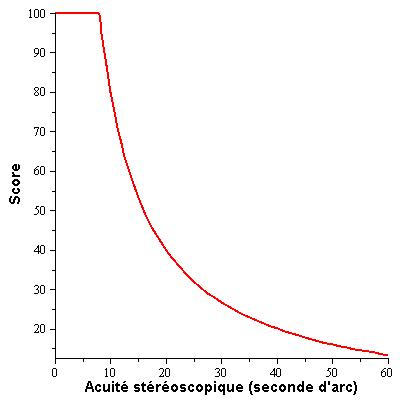
\includegraphics[scale=.9]{Figures/StereoAcuity}
		\caption{Tracé de la fonction de notation du critère <<~acuité stéréoscopique~>> ($\Delta \nu_{min} = 8~arcsecs$)}
		\label{fig:stereo_acuity}
	\end{figure}